\documentclass[First Project.tex]{subfiles}
\begin{document}

\subsection{ Τροποποιημένη μέθοδος της διχοτόμησης }

Στην τροποποιημένη μέθοδο της διχοτόμησης αυτό που αλλάζει είναι ο τρόπος που γίνεται η εκτίμηση της ρίζας από μία γεννήτρια παραγωγής 
τυχαίων αριθμών ενώ οι προϋποθέσεις της μέθοδου παραμένουν ίδιες. Η συνάρτηση \textit{\textlatin{\textbf{modified\_bisection}}} από το αρχείο 
\textit{\textlatin{\textbf{modified\_bisection.py}}} δέχεται τα ίδια ορίσματα με την κλασσική μέθοδο της διχοτόμησης, ενώ η εκτίμηση της ρίζας
γίνεται από μία γεννήτρια παραγωγής τυχαίων αριθμών από ομοιόμορφη κατανομή. Ακόμα, αλλάζει ο τρόπος υπολογισμού του σφάλματος σε κάθε βήμα
και οι επαναλήψεις συνεχίζονται μέχρι το μήκος του διαστήματος \textlatin{\textbf{[a,b]}} να γίνει μικρότερο από το σφάλμα \textlatin{\textbf{eps}}, με
αυτό τον τρόπο το μεγαλύτερο σφάλμα που μπορεί να γίνει από την γεννήτρια παραγωγής τυχαίων αριθμών είναι \textlatin{\textbf{eps}}, που είναι
το επιθυμητό.Επομένως, έχουμε για την ρίζα στο διάστημα \textbf{[0.5,1.0]} τα παρακάτω :
\vspace{5px}
\begin{figure}[h!]
    \centering
    \captionsetup{justification=centering}
    \begin{center}
        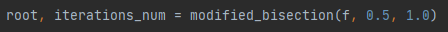
\includegraphics[scale=1]{exercise_2_bisection_call_first_root.png}    
        \caption{Παράδειγμα κλήσης της συνάρτησης \textit{\textlatin{\textbf{modified\_bisection}}}.}
    \end{center}
\end{figure}


Μετά την κλήση της συνάρτησης \textit{\textlatin{\textbf{modified\_bisection}}} τα αποτελέσματα είναι τα εξής:
\vspace{5px}
\begin{figure}[h!]
    \centering
    \captionsetup{justification=centering}
    \begin{center}
    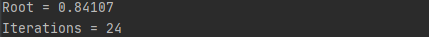
\includegraphics[scale=1]{exercise_2_bisection_results_first_root.png}    
    \caption{ Αποτελέσματα κλήσης της συνάρτησης \textit{\textlatin{\textbf{modified\_bisection}}} \\ στο διάστημα \textbf{[0.5,1.0]}. }
    \end{center}
\end{figure}

Ώπου παρατηρούμε ότι η ρίζα της \textlatin{\textbf{f(x)}} στο διάστημα \textbf{[0.5,1.0]} με ακρίβεια 5 δεκαδικών ψηφίων 
είναι η \textbf{0.84107} καθώς και ότι η τροποποιημένη μέθοδος της διχοτόμησης χρειάστηκε \textbf{24} επαναλήψεις για να επιτύχει την 
επιθυμητή ακρίβεια. Για την ρίζα της συνάρτησης στο διάστημα \textbf{[1.0,1.25]} έχουμε 
\vspace{5px}
\begin{figure}[h!]
    \centering
    \captionsetup{justification=centering}
    \begin{center}
        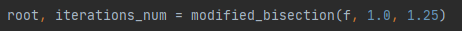
\includegraphics[scale=1]{exercise_2_bisection_call_second_root.png}    
        \caption{Παράδειγμα κλήσης της συνάρτησης \textit{\textlatin{\textbf{modified\_bisection}}}.}
    \end{center}
\end{figure}


Μετά την κλήση της συνάρτησης \textit{\textlatin{\textbf{modified\_bisection}}} τα αποτελέσματα είναι τα εξής:
\vspace{5px}
\begin{figure}[h!]
    \centering
    \captionsetup{justification=centering}
    \begin{center}
    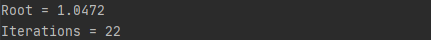
\includegraphics[scale=1]{exercise_2_bisection_results_second_root.png}    
    \caption{ Αποτελέσματα κλήσης της συνάρτησης \textit{\textlatin{\textbf{modified\_bisection}}} \\ στο διάστημα \textbf{[1.0,1.25]}.}
    \end{center}
\end{figure}

Ώπου παρατηρούμε ότι η ρίζα της \textlatin{\textbf{f(x)}} στο διάστημα \textbf{[1.0,1.25]} με ακρίβεια 5 δεκαδικών ψηφίων 
είναι η \textbf{1.0472} καθώς και ότι η τροποποιημένη μέθοδος της διχοτόμησης χρειάστηκε \textbf{22} επαναλήψεις για να επιτύχει την 
επιθυμητή ακρίβεια. Στην συνέχεια παρατηρούμε ότι η τελευταία ρίζα της συνάρτησης βρίσκεται στο διάστημα \textbf{[2.0,2.5]}, αν υπολογίσουμε
τις τιμές της συνάρτησης στα άκρα του διαστήματος έχουμε 
\begin{equation*}
    f(2.0) * f(2.5) = 15.018 * -31.305 = -470.13 < 0
\end{equation*} 

οπότε σύμφωνα με το θεώρημα \textlatin{\textbf{Bolzano}} η συνάρτηση όντως έχει μία ρίζα σε αυτό το διάστημα.
\vspace{5px}
\begin{figure}[h!]
    \centering
    \captionsetup{justification=centering}
    \begin{center}
        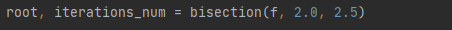
\includegraphics[scale=1]{exercise_2_bisection_call_third_root.png}    
        \caption{Παράδειγμα κλήσης της συνάρτησης \textit{\textlatin{\textbf{modified\_bisection}}}.}
    \end{center}
\end{figure}


Μετά την κλήση της συνάρτησης \textit{\textlatin{\textbf{modified\_bisection}}} τα αποτελέσματα είναι τα εξής:
\vspace{5px}
\begin{figure}[h!]
    \centering
    \captionsetup{justification=centering}
    \begin{center}
    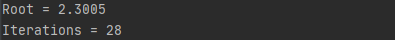
\includegraphics[scale=1]{exercise_2_bisection_results_third_root.png}    
    \caption{ Αποτελέσματα κλήσης της συνάρτησης \textit{\textlatin{\textbf{modified\_bisection}}} \\ στο διάστημα \textbf{[2.0,2.5]}.}
    \end{center}
\end{figure}

Ώπου παρατηρούμε ότι η ρίζα της \textlatin{\textbf{f(x)}} στο διάστημα \textbf{[2.0,2.5]} με ακρίβεια 5 δεκαδικών ψηφίων 
είναι η \textbf{2.3005} καθώς και ότι η τροποποιημένη μέθοδος της διχοτόμησης χρειάστηκε \textbf{28} επαναλήψεις για να επιτύχει την 
επιθυμητή ακρίβεια.
\end{document}